\documentclass[12pt,a4paper]{article}
\usepackage[utf8]{inputenc}
\usepackage{amsmath}
\usepackage{amsfonts}
\usepackage{amssymb}
\usepackage[left=2cm,right=2cm,top=2cm,bottom=2cm]{geometry}
\usepackage{tikz}
\usetikzlibrary{automata, arrows.meta, positioning}

\author{Hao Ran}
\title{Generative equations of the Nee Soon IBM}

\begin{document}
\maketitle

Let's write down the Nee Soon individual-based model (IBM) mathematically since we will inevitably need to do so in the manuscript. I tried my best to transcribe the R codes and our verbal communication mathematically but something may be incorrect. Need to double check.

\section{Transitional diagram}

A draft state diagram of the IBM. Initial seedling and adult numbers and diameters are determined [...] Edge labels are vital rates parameterised with regression and field data... Vital rates are influenced by stand competition, habitat mismatch, or both, as determined by model selection.

\begin{center}
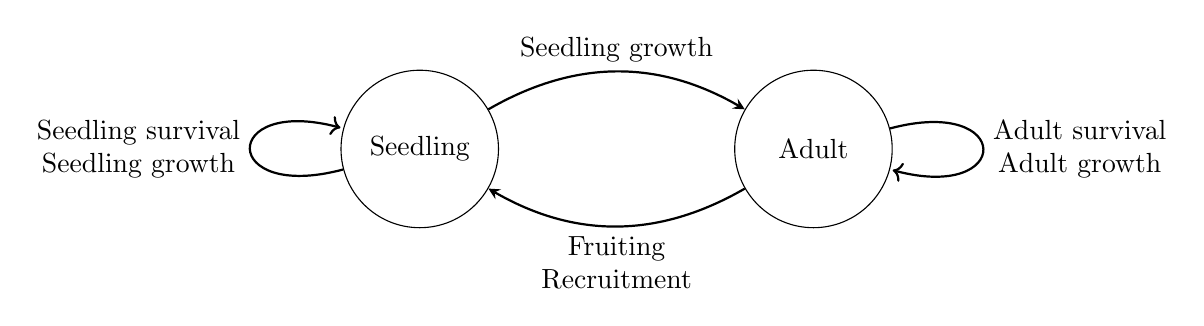
\begin{tikzpicture} [node distance = 5cm, on grid, auto, state/.style={circle, draw, minimum size=2cm}]
\node (s) [state, ] {Seedling};
\node (a) [state, right = of s] {Adult};
\path [-stealth, thick]
    (s) edge [bend left] node [above] {Seedling growth} (a)
    (a) edge [bend left] node [below, align=center] {Fruiting \\ Recruitment} (s)
    (a) edge [loop right] node [align=center] {Adult survival\\ Adult growth} ()
    (s) edge [loop left] node [align=center] {Seedling survival\\ Seedling growth} ();
\end{tikzpicture}
\end{center}

\section{Fruiting incidence}
For tree individual $i$ of species $j$ with diameter-at-breast-height, $D_{ij}$, in a spatial grid $p$ with habitat index, $H_p$, at time point $t$, we model its fruiting incidence [yes or no] in the subsequent time point as a Bernoulli process with mean $p_{\text{fruit},ijp}$, which is a linear function of the species-specific potential fruiting incidence $\phi_{0,j}$, species-specific size dependence $\phi_{D,j}$, and overall effect of habitat mismatch, $\phi_H$:
\begin{align}
\Pr\left(\text{Fruiting}_{ij,p,t+1}=1\right) &\sim \text{Binomial}\left(1,~p_{\text{fruit},ij,p,t+1}\right) \\
\text{logit}\left(p_{\text{fruit},ij,p,t+1}\right) &= \phi_{0,j} + \phi_{D,j} D_{ij,p,t} + \phi_H \Delta H_{ij,p,t} \,.
\end{align}
The habitat mismatch, $\Delta H_{ij,p,t}$, of an individual is measured as [...]

\section{Seedling recruitment}
For each parent tree that fruited, we model its offspring count as a size-dependent power function with mean $r_{ij,t+1}$ and dispersion $\psi_j$:
\begin{align}
R_{ij,t+1} &\sim \text{NegBinom}\left(r_{ij,t+1},~\psi_j\right) \\
r_{ij,t+1} &=  \rho_{0,j} D_{ij,t}^{\rho_{D,j}} \label{eq:fruit} \\
\log\left(r_{ij,t+1}\right) &=  \log \rho_{0,j} + \rho_{D,j} \log D_{ij,t} \,
\end{align}

\section{Seedling location}
We allow newly-recruited seedlings to follow a species-specific `2DT' dispersal kernel (REF), which has the probability density function (PDF):
\begin{equation}
\frac{\Sigma_j}{\pi \Lambda_j \left(1 + \frac{d^2}{\Lambda_j}\right)^{\Sigma_j+1}} \,,
\end{equation}
where $d$ is the distance from a parent tree. Because this PDF does not have a closed form, we numerically sample $d$ from this PDF after normalising the PDF to sum to one for $d \in (0, 410)$ meters.

\textit{Note: changed latin letters to Greek to reserve $S$ for survival}

\section{Seedling growth and survival}
For each seedling we model its size-dependent survival $S_{\text{seedling},ij,p,t+1}$ following Needham et al. (2018):
\begin{align}
\Pr(S_{\text{seedling},ij,t+1} = 1) &\sim \text{Binomial}(1,~s_{ij,t+1}) \\
s_{ij,t+1} &= \dfrac{K_j}{1 + e^{-r_{1,j}  (D_{ij} - p_{1,j})}} \,, 
\end{align}
where seedling diameter $D_{ij}$ is converted from height (because seedling growth is calculated as height increment, see below):
\begin{align}
\log D_{ij} &\sim \text{Normal}(\mu_{\log D,ij},~\sigma_{\log D}) \\
\mu_{\log D,ij} &= d_{0,j} + d_{H,j} \log H_{ij}
\end{align}
\textit{Note: currently diameter is not generated with variance, but only deterministically using the linear predictor!}

For each surviving seedling we model its subsequent log height $\log H_{ij,t+1}$ as a function of previous log height, conspecific competition, heterospecific competition, and their interactions:
\begin{align}
\log H_{ij,t+1} \sim~& \text{Normal}(\mu_{\log H, ij,t+1},~\sigma_{\log H}) \\
\mu_{\log H, ij,t+1} =~& h_{0,j} + h_{H,j} \log H_{ij,t+1} + h_{\text{intra},j}\text{Consp}_{i,t} + h_{\text{inter},j}\text{Hetsp}_{i,t} \\
& + h_{\text{intra}H,j}\log H_{ij,t+1}\text{Consp}_{i,t} + h_{\text{inter}H,j}\log H_{ij,t+1}\text{Hetsp}_{i,t} \\
\text{Consp}_{i,t} =~& ??? \\
\text{Hetsp}_{i,t} =~& ???
\end{align}

\section{Adult growth}
The size-dependent annual diameter growth $G_{ij,p,t}$ of adults follows Zeide (1993) and Kohyama et al. (2020):
\begin{align}
D_{ij,p,t+1} &= D_{ij,p,t} + G_{ij,p,t}\\
G_{ij,p,t} &\sim \text{Normal}(\mu_{G,ij,p,t},~\sigma_{G}) \\
\mu_{G,ij,p,t} &= D_{ij,p,t}^{b} e^{a-c D_{ij,p,t}} \\
a &= a_j + a_{\text{intraA},j} \text{intraA}_{i,t} + a_{\text{interA},j} \text{interA}_{i,t} + a_{\text{H},j} \Delta H_{p,t} \\
b &= b_j \\
c &= c_j + c_{\text{intraA},j} \text{intraA}_{i,t} + c_{\text{interA},j} \text{interA}_{i,t} + c_{\text{H},j} \Delta H_{p,t}
\end{align}

\section{Survival}
Finally, we model survival individuals of all sizes, i.e., `seedlings' and `adults'. Seedling sizes (which have the units of log height in the model) are first converted to log DBH units via extrapolation of the seedling diameter--height allometric equation as above.

Then, the following survival model from Needham et al. (2018), we predict the probability of survival of each individual based on its size (in log DBH units)
\begin{align}
\Pr(S_{\text{adult},ij,p,t+1} = 1) &\sim \text{Binomial}(1,~s_{\text{adult},ij,p,t+1}) \\
s_{\text{adult},ij,p,t+1} &=
    \dfrac{K_j}{1 + e^{-(r_{10,j} + r_{11,j} \cdot \text{interA}_{i,t} \cdot \Delta H_{ip,t}) [D_{ij} - (p_{10,j} + p_{11,j} \cdot \text{intraA}_{i,t}) ]}} \\
\text{intraA}_{i,t} &= ??? \\
\text{interA}_{i,t} &= ???
\end{align}


\textit{Note: some random intercepts potentially are missing from all the equations above; need to double check}

\section{References}

\noindent Kohyama, T. S., Potts, M. D., Kohyama, T. I., Niiyama, K., Yao, T. L., Davies, S. J., \& Sheil, D. (2020). Trade-off between standing biomass and productivity in species-rich tropical forest: Evidence, explanations and implications. \textit{Journal of Ecology}, 108(6), 2571–2583. doi: 10.1111/1365-2745.13485
\\

\noindent Needham, J., Merow, C., Chang-Yang, C.-H., Caswell, H., Mcmahon, S. M., \& Needham, J. (2018). Inferring forest fate from demographic data: from vital rates to population dynamic models. \textit{Proceedings of the Royal Society B: Biological Sciences}, 285(1874), 20172050. doi: 10.1098/rspb.2017.2050
\\

\noindent Zeide, B. (1993). Analysis of growth equations. \textit{Forest Science}, 39(3), 594–616. doi: 10.1111/j.1461-0248.2006.00883.x
\end{document}
